%% main text
\chapter{Macroscopic Approximation methods for networked agent-based models}
\label{chapter:approximation}
In this chapter, I develop a method to find approximate solutions to heterogeneous-agent models with interactions that happen pair wise as well as on a mean field level. To introduce, I elaborate on the implications that this has for the use of agent-based models in economics in section \ref{sec:approx_intro}. I develop the method at hand of a simplification of the model that I introduced in section \ref{sec:heuristics_model} and will give a short recap of the simplified model specifications in section \ref{sec:approx_Model_Description}. I give a detailed explanation of the method in section \ref{sec:Approximation} and illustrate one of its advantages by doing a bifurcation analysis of the approximated model in section \ref{sec:bifurcation-analysis} before concluding. 
\section{Introduction}
\label{sec:approx_intro}

% Introduction to agent-based models
Agent-based modeling is a computational approach to simulate systems composed of a large number of similar sub-units with many applications in ecology \citep{Grimm2005}, business \citep{Bonabeau2002}, sociology \citep{Macy2002} and economics \citep{Tesfatsion2006, Hamill2015}.
ABMs are used to study aggregate phenomena emerging from local interactions \citep{Epstein1999}.
These interactions can be structured by spatial embedding of agents or by social networks \citep{Gross2008,Holme2006a,Bargigli2014}.

% applications in economics
In economics, ABMs have been used to study for example business cycles \citep{DelliGatti2008}, market power \citep{Tesfatsion2006} and trade \citep{Hamill2015}.

% Introduction to macroeconomic modeling and the aggregation problem
ABMs are a promising alternative to dynamic stochastic general equilibrium (DSGE) modeling, the current workhorse of theoretical macroeconomics. 
DSGE models usually build on the representative agent approach, i.e., they represent all individuals of one type such as firms or consumers by one representative decision maker.
%to hold up to Lucas' influential critique that macroeconomic model should not use statistical correlations between aggregate variables but rather build on the behavior of individual economic agents \citep{Janssen2016, Lucas1976}.

% Disadvantages/critique of representative agent, 
% pros and cons of DSGEs
% cons:
The representative-agent approach implies that theoretical macroeconomics reduces macroeconomic phenomena to assumptions about a few different representative agents, leaving out many explanatory mechanisms for fluctuations in aggregate variables based on intra-group interaction and heterogeneity.\footnote{Approaches to represent heterogeneous agents in DSGE models have been used to counter this criticism and add more realism regarding the distribution of agent attributes \citep[see for example the review by][]{Heathcote2009}.
Particularly, because the representative agent approach cannot account for interactions within a heterogeneous group, models using this approach do not allow for the representation of emergent phenomena \citet{Kirman1992}.\footnote{I use here a weak notion of emergence, which allows explaining macro-phenomena on the basis of micro-interactions of the systems constituents that differ from the explained macro-phenomena. This is opposed to strong emergence, that embraces the irreducibility of macro-phenomena to lower-level dynamics. For a discussion see \citet{Bedau1997}.}
But their solution require complex numerical methods and cannot integrate local interactions between agents.}
Furthermore, DSGE model often assume rational expectations, i.e., agents know the constraints and dynamics of the entire economy which has been criticised as philosophically unsound and empirically unjustified \citep{Kirman2014}.
% pros:
But, due to these assumptions, most DSGEs allow for a thorough analytical analysis.

% pros and cons of ABMs:
% pros:
ABMs allow implementing various individual decision models that are behaviorally more realistic than full economic rationality.
Agents are often assumed to be boundedly rational and adapt their expectations, which is compatible with the Lucas critique \citep{Evans2006}.
In ABMs, fluctuations in aggregate variables do not only arise from exogenous shocks as in DSGE models but primarily from irregularities in local interactions.
Therefore, they offer an avenue for explaining various emergent phenomena studied in empirical macroeconomics.

% cons:
On the other hand, ABMs are often very detailed so that an analytic treatment is unfeasible. 
Therefore, in ABMs, the difficulties arising from the aggregation of heterogeneous and interacting agents are usually solved computationally.
Because the model mechanisms are difficult to trace in the `black box' of a computational model, the results of ABMs are often difficult to interpret and cannot provide mathematically sound proofs of relationships between model variables. Results may therefore be difficult to generalize \citep{Leombruni2005}.
There has been some progress in the standardization of model descriptions for ABMs \citep{Grimm2006}, but the lack of standardization, e.g., of decision rules, makes the models difficult to compare \citep[][p. 239]{Hamill2015}. Even though there are various techniques available for comprehensive model analysis \citep{Lee2015}, a systematic model exploration is uncommon and mostly limited to sensitivity analysis with respect to crucial parameters.

% Bringing the two together
Methods from theoretical physics have been applied successfully to various problems in economics for many years \citep{Mantegna1999}. Here, aggregation methods from statistical physics can bridge the gap between analytic macroeconomic models such as DSGE approaches and agent-based computational models \citep[for a review of physics methods in social modeling, see ref.][]{castellano2009statistical}. In contrast to macroeconomic models, these approaches account for local interactions and use aggregation techniques to derive macro-dynamics, providing a true microfoundation of the resulting macromodel.
These kinds of approximation methods have found much interest in the fields of financial economics, behavioral finance and evolutionary game theory recently and have produced interesting and promising results, e.g., to explain macroeconomic fluctuations and understand propagation of financial shocks and the resulting systemic risk.

%short discussion of some of the work already done in this field

% include this literature as well?
%Di Guilmi et al. 2012 (SSRN): Credit network economy, analytical approximation via Master equation
%Delli Gatti et al. 2005 (JEDC): interacting agents, mention of network but use unclear
%Gualdi et al. 2015 (JEDC): Analysis of Delli Gatti model (see books) in phase space, identification of tipping behavior
% \citep{DelliGatti2008}: stochastic aggregation very general and not related to networks

Many authors use mean field approximations to study interactions between heterogeneous agents, e.g., making use of Master and Fokker-Planck equations \citep{Aoki1998, Aoki2007, DelliGatti2000, DiGuilmi2008, Chiarella2011a, Landini2014}. Such approaches assume that each agent pair interacts with the same probability.
But many social and economic interactions are structured and the structure can be described by complex networks \citep{Friedkin2011}. Therefore, some approximation methods take network structure into account and derive macroscopic quantities that describe the structure of networks \citep[e.g.][]{Alfarano2008a, Lux2016}.

Yet, most of the literature regards either the network between agents or the states of agents as static, implicitly assuming different time scales for dynamics of and processes on the network.
However, recent literature on opinion formation processes and the spreading of social norms in the field of computational social sciences suggests that both happen on a comparable timescale and can therefore not be treated separately \citep{Gross2008, gross2009adaptive}.
A typical example of a model that takes this into account is the one that I present in this paper. I use this model to demonstrate how the individual techniques mentioned above may be combined. In this model, the network of interactions between agents as well as the spreading of behavior between agents on this interaction network happen on a comparable timescale.
For such adaptive networks \citep{Gross2008}, moment closure techniques have been introduced in the physics literature to aggregate the feedback between complex adaptive network dynamics and dynamics of single node states \citep{Do2009, Demirel2014, Wiedermann2015, Min2017}.
Here, I introduce these techniques to economic modeling and combine them with approaches from macroeconomics where interactions also happen globally via aggregated variables.

% Discussion of usefulness of analytic approximations
The technical challenges of analytic approximation methods for agent-based model has so far hampered their wide-spread use in economics. But they have a huge potential in providing profound insights into dynamical properties of economic systems: First, they help increasing performance of computer simulations, making calculation of single model runs much faster and therefore allowing for a wider range of bifurcation and parameter analyses. Second, in contrast to stochastic simulations, they make formal proofs of relations between macroscopic variables possible. Third, they allow the derivation of analytical expressions of relations between model variables from the dynamic equations, which is not possible from single simulation runs. This paper makes a step forward in showcasing how such methods can be used to combine interactions on complex adaptive networks with macroeconomic modeling. It is therefore a contribution to integrate non-standard behavioral assumptions into macroeconomic models.

% Contribution of this paper % Introduce the model in the paper
The agent-based model I use for the illustration of these methods comes from the context of climate economics to show how these approximation techniques can be applied to models that combine local interactions on a network with system-level interactions through markets.
In particular, I use moment closure, pair, and large system limit approximations to derive an aggregate description for the dynamics of my model.
The model consists of heterogeneous households that interact and learn from neighbors on a social network and a two-sector productive economy.
The households differ in their investment strategy: they invest their savings either in the ``dirty'' or the ``clean'' sector, each representing a separate capital market through which the agents interact.
Agents imitate the investment strategy of acquaintances that are better off with a higher probability.
To the best of my knowledge this is the first study that applies such a combination of approximation methods on a model that combines structured local with global interactions of heterogeneous agents in a socioeconomic setting.
Self-evidently, despite the fact that the reference application is an economic one, this approximation method can also be used to describe similarly structured models in other fields of research such as social-ecology, neuroscience or computational social science.

% Outline
In the following section, I give a specification of the model that I use to illustrate the approximation method. The model is a simplification of the one introduced in section \ref{sec:heuristics_model}. I will therefore not discuss its details again but only give a short recap of its specifications and elaborate on the simplifications.
%In the remainder of the paper, I first describe the details of the model (Sec.~\ref{sec:approx_Model_Description}). Then, I derive an aggregate description of the model by applying three approximation techniques, moment closure, pair approximation, and large system limit (Sec.~\ref{sec:Approximation}). I discuss commonalities and differences between computer simulations and the approximation approach. Before concluding, I illustrate how the derived macro-approximation can be used in a bifurcation analysis to better understand the qualitative properties of the non-linear model (Sec.~\ref{sec:bifurcation-analysis}).

\section{Model Description}
\label{sec:approx_Model_Description}

To illustrate the application of the methods that I put forward, I use a model of a stylized two sector investment economy that captures the shift from fossil-fuel to renewable energy-based based production. Essentially, this equals the model that I introduced in section \ref{sec:heuristics_model} with the difference that I abstract from the separation of judgement and actions in terms of a heuristic decision model. Instead, households decisions whether to invest in one or the other sector are directly governed by the adaptive voter dynamic.
Consequently, if the reader still has the model in mind, they can safely skip the model description and continue with section \ref{sec:numerical_results} where I present first results.

This model is designed to incorporate the dynamics of social norms that underlie investment decisions in the context of climate economics and policy. Decarbonization pathways consistent with the Paris agreement require a rapid shift of investments away from fossil fuel exploration and extraction to the development and deployment of renewable energies \citep{IPCC2014}. However, the implementation of climate policies is uncertain and expectations cannot be based on self-consistent beliefs about the future.  In conventional macroeconomic models such shifts can only occur due to price signals either from improvements in green technology, increasing scarcity of fossil reserves, or carbon pricing. While price signals are certainly important, movements advocating for the divestment from fossil fuels point to the role of social norms and practices regarding investment decision to initiate and accelerate the energy transition \citep{Ans2013}. To better understand such culturally driven situations of socioeconomic change, it is important to work with models that can incorporate endogenous preferences and aspects of bounded rationality such as imperfect foresight and information as well as learning.
%\begin{figure}[t]
%  \centering
%  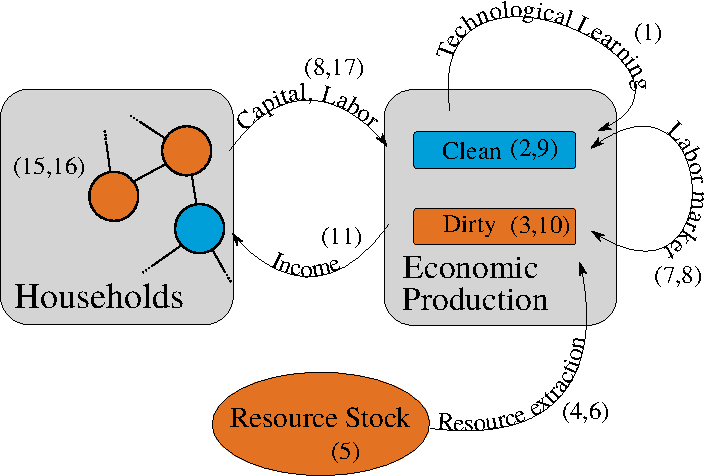
\includegraphics[width=.8 \textwidth]{figures/model_scheme.pdf}
%\caption{Schematic figure of the model consisting of two production sectors of which one depends on an exhaustible fossil resource stock as well as a set of heterogeneous households that interact on an adaptive complex network and use social learning to decide upon which of two production sectors to invest in. Boxes and bubbles denote modeled entities, arrows denote interactions. Numbers in brackets $(x)$ refer to equations $(6.x)$ that describe the specific part of the model.}
%  \label{fig:model_scheme}
%\end{figure}
% \subsection{Economic Production}
\label{sec:approx_economy}

The underlying assumptions of the economic model are discussed in detail in section \ref{sec:heuristics_model}. This is a brief recap of the specifications of the economic production model. 

The model consists of two sectors for production and a set of heterogeneous households that interact via a complex adaptive social network. The two production sectors employ different technologies where the production technology in one sector depends on the input of an exhaustible (fossil) energy-resource $R$ that is used up in the process whereas the technology in the other sector does not. They are called the \textit{dirty} and the \textit{clean} sector accordingly. Capital is technology specific and can not be reallocated between the two sectors.
Therefore, the heterogeneous households in the model provide different types of capital $K_j$ as well as labor $L$ to the sectors.
The technology in the dirty sector is fully developed and adequately described in terms of the total factor productivity. 

The clean sector represents a circular economy in which the output of final goods depends on the machinery, knowledge and effort used in its production and is not limited by entropy laws or resource scarcity on the timescale under consideration. The technology $C$ used in the clean sector is assumed to be still in development and is therefore explicitly modeled.
Technological progress is implemented as learning by doing according to Wright's law \citep{wright1936factors, Nagy2013} with a one-factor learning curve. $C$ is proportional to cumulative production but also depreciates with a constant rate $\chi$.

\begin{equation}
	\dot{C} = Y_c - \chi C.
	\label{eq:approx_lbd}
\end{equation}

Capital, labor and technology/knowledge are mutual substitutes. The production functions $Y_c = b_c C^{\gamma} L_c^{\alpha_c}K_c^{\beta_c}$  for the clean and 	$Y_d = \mathrm{ min}\left( b_d L_d^{\alpha_d}K_d^{\beta_d}, e R \right),$ for the dirty sector satisfy these requirements. Subscripts $c$ and $d$ denote the clean and dirty sector respectively, $L_c$ and $L_d$ are labor shares, $\alpha$ and $\beta$ are elasticities of the respective input factors, $b_c$ and $b_d$ are the total factor productivity and $K_c$ and $K_d$ are the capital stocks for the respective sector.
The dirty sector uses the resource efficiently, such that
\begin{equation}
    b_d L_d^{\alpha_d}K_d^{\beta_d} = e R
    \label{eq:approx_edr}
\end{equation}
where $1/e$ is the resource intensity of the sector. The usage of the fossil resource $R$ depletes a geological resource stock $G$ with the initial stock $G(t=0) = G_0$:
\begin{equation}
    \dot{G} = -R. 
    \label{eq:approx_rdep}
\end{equation} 
The total cost $c_R$ for the usage of the fossil resource depends on the resource use $R$ and the remaining fossil resource stock $G$ as $c_R = b_R R^{\rho}\left( \frac{G_0}{G} \right)^{\mu}$ with $\rho \geq 1$ and $\mu > 0$ such that $\partial c_R / \partial R >0$ and $\partial c_R / \partial G < 0$.
This means that at some point $\partial Y_d / \partial R < \partial c_R / \partial R$ to take into account that some part of the resource is not economic, e.g. its marginal cost exceeds its marginal productivity.
The equilibrium wage $w$ equals the marginal return for labor:
\begin{equation}
	w = \frac{\partial Y_c}{\partial L_c} = \frac{\partial Y_d}{\partial L_d} - \frac{\partial c_R}{\partial L_d}
	\label{eq:approx_equilibrium_wage}
\end{equation}
with the sum of the labor shares equal to the total amount of labor available:
\begin{equation}
	L_c + L_d = L.
	\label{eq:approx_L}
\end{equation}
Capital rents equal marginal productivity e.g., 
\begin{align}
  r_c &= \frac{\partial Y_c}{\partial K_c}, \label{eq:approx_ccr}\\
  r_d &= \frac{\partial Y_d}{\partial K_d} - \frac{\partial c_R}{\partial K_d}. \label{eq:approx_dcr}
\end{align}

\subsection{Adaptive Network Model for Investment Decision Making}
\label{sec:investment_decision_making_descr.}
%\JJK{Maybe comment on the relationship between individual optimization, group level optimization and the imitation of successful strategies.}
For the approximation methods derived here, I have do abstract from the separation of judgment and actions that I proposed in section \ref{sec:investment_decision_making} [TODO: also cite part of general introduciton].
Still, I model households as bounded rational decision makers \citep{simon1972theories, simon1982models, gigerenzer2002bounded}.
That is, households take their investment decisions, i.e. whether to invest their savings in the clean or the dirty sector, not by forming rational expectations \citep{Evans2006, Kirman2014} but by engaging in social learning \citep{Bandura1971} to obtain successful strategies \citep{Traulsen2010} with reasonable effort.
As the outcomes of social learning crucially depend on the structural properties of the complex network of social ties amongst the households \citep{Barkoczi2016}, I model the adaptive formation of this social network endogenously.
A well established principle for the emergence of structured ties in social networks is homophily, i.e. the tendency that similar individuals are linked \citep{McPherson2007, Centola2007, Centola2011}.
The following model specification uses social learning in combination with endogenous network formation based on homophily to model the investment decisions of the households.

I model $N$ heterogeneous households denoted with the index $i$ as owners of one unit of labor $L^{(i)} = L/N$ and capital $K_c^{(i)}$ and $K_d^{(i)}$ in the clean and dirty economic sector respectively.
Households generate an income $I^{(i)}$ from their labor and capital income which they use for consumption $F^{(i)}$ and savings $I^{(i)}$:
\begin{align}
	I^{(i)} &= w L^{(i)} + r_c K_c^{(i)} + r_d K_d^{(i)}, \label{eq:approx_hi} \\
	F^{(i)} &= (1-s) I^{(i)}, \label{eq:approx_c} \\
	S^{(i)} &= s I^{(i)}. \label{eq:approx_s}
\end{align}
A binary decision parameter $o_i \in [c,d]$ denotes the sector in which the households decide to invest. As motivated above, I model decision making that is driven by two processes: social learning via the imitation of successful strategies and homophily towards individuals exhibiting the same behavior. \\
I describe households as the nodes in a graph of acquaintance relations that follow the following rules. 
\begin{enumerate}
  \item Households get active at a constant rate $1/\tau$. \label{r1}
        \item When a household $i$ becomes active, it interacts with one of its acquaintances $j$ chosen uniformly at random. 
        \item If they follow the same strategy, i.e. they invest in the same sector, nothing happens. 
        \item If they follow a different strategy, i.e. they invest in different sectors, one of two actions can happen:
        \begin{enumerate}
                \item Homophilic network adaptation: with probability $\varphi$, the households end their relation and household $i$ connects to another household $k$, that follows the same strategy. 
                \item Imitation: with probability $1-\varphi$, household $i$ engages in social learning i.e. it imitates the strategy of household $j$ with a probability $p_{ji}$ that increases with their difference in income. \label{rn}
        \end{enumerate}
\end{enumerate}
I follow previous results on human strategy updating in repeated interactions from \cite{Traulsen2010}, when I assume the imitation probability as a monotonously increasing function of the relative difference in consumption between both households:
\begin{equation}
	p_{ji} =  \left(1 + \exp \left(- \frac{a(F^{(i)} - F^{(j)})}{F^{(i)} + F^{(j)}} \right) \right)^{-1}.
    \label{eq:approx_ip}
\end{equation}
As opposed to the absolute difference in the original study by \cite{Traulsen2010}, the probability in this model depends on relative differences. 
I set $a = 8$ to conform to their empirical evidence. This dependence on relative differences in per household quantities is crucial for my method as I will discuss later at the end of sec. \ref{sec:large_system_limit}.
I model strategy exploration as a fraction $\varepsilon$ of events that are random, e.g. rewiring to a random other household or randomly investing in one of the two sectors.
Given the savings decisions of the individual households, and assuming equal capital depreciation rates $\kappa$ in both sectors, the time development of their capital holdings is given by

\begin{align}
	\dot{K}_c^{(i)} =& \delta_{o_ic} \left( r_c K_c^{(i)} + r_d K_d^{(i)} + w L_i \right) - \kappa K_c^{(i)} \label{eq:approx_ci}\\
	\dot{K}_d^{(i)} =& \delta_{o_id} \left( r_c K_c^{(i)} + r_d K_d^{(i)} + w L_i \right) - \kappa K_d^{(i)} \label{eq:approx_di}
\end{align}

where $\delta_{ij}$ is the Kronecker Delta. The total capital stocks in the two sectors are made up of the sum of the individual capital stocks as
\begin{equation}
K_j = \sum_i^N K_j^{(i)} = N k_j,
\end{equation}
where $k_j$ is the average per household capital stock of a given capital type.

I acknowledge the fact that different model specifications are possible and interesting.
For instance, I only consider fixed savings rates and the decision between two capital assets and leave the analysis of the interesting possible effects of households setting their savings rates individually to another study \citep{Asano2019}.
However, I want to point out that the approximation methods that I develop in the following are highly useful to gain insights from different but similar models that rely on complex adaptive interaction networks.


   
\subsection{Numerical Modelling and Results} 
\label{sec:numerical_results}
\textcolor{red}{I think that this subsection is a candidate for removal.}\\

% JK: distinguish better between assumptions, initial conditions and findings/results.
With the model specifications from sec. \ref{sec:approx_Model_Description}, the parametrization in Tab.~\ref{tab:Parameter_list} and appropriate initial conditions for the dynamic variables, the model can be simulated numerically.
For this, I implemented the dynamics in the multi-purpose programming language python. The implementation of the ABM as well as the numerical analysis using the approximation methods described in the following are available on github in \cite{kolb2018}.
In the following, I discuss the resulting aggregate dynamics.

\begin{figure}[ht]
  \centering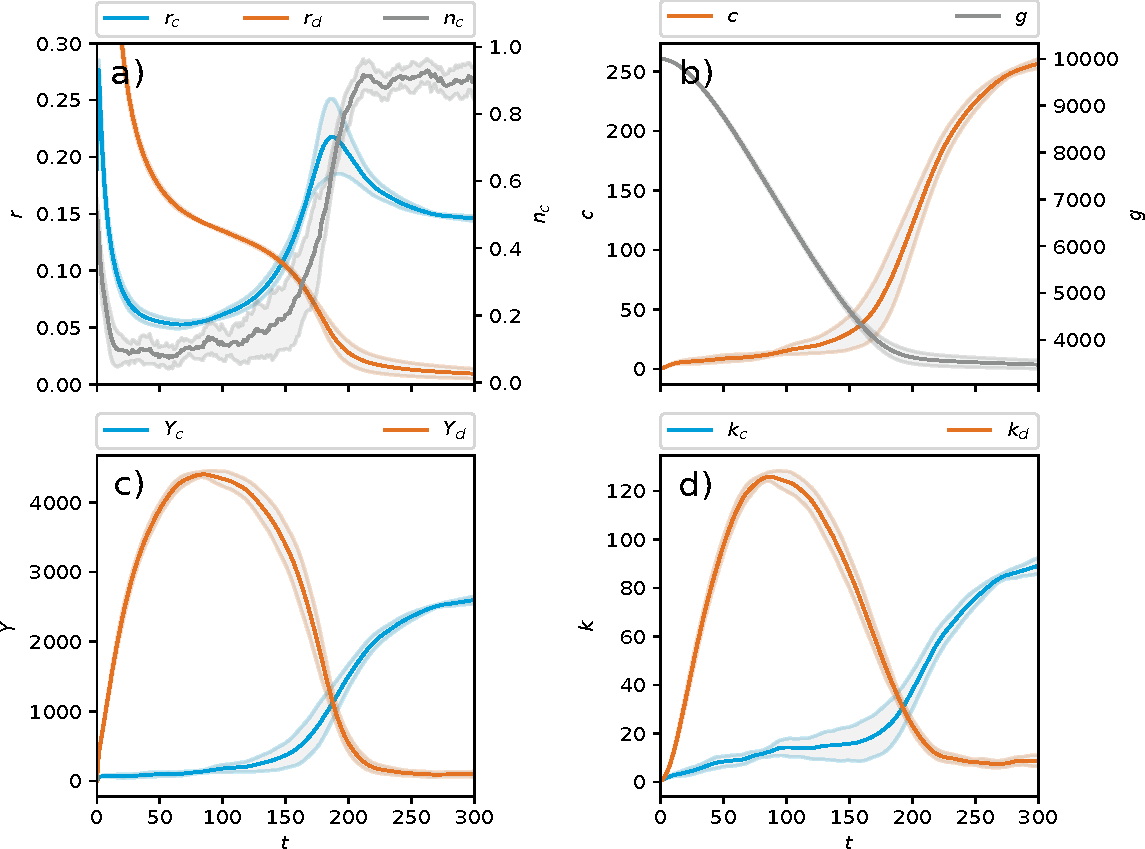
\includegraphics[width=.85\linewidth]{figures/example_trajectory.pdf}
  \caption{\textbf{Example trajectory of the ABM.} Solid lines show mean results from 100 runs of the model in per capita variables. Grey areas around solid lines show their standard deviation. The panels show capital rents in the clean and dirty sector $r_c$ and $r_d$ as well as the fraction of households investing in the clean sector $n_c$ in panel a, knowledge and resource stock $c$ and $g$ in panel b, output of clean and dirty sector $Y_c$ and $Y_d$ in panel c and per capita capital $k_c$ and $k_d$ in the clean and dirty sector (d).
Initial conditions are $G=G_0$, $C=1$, $K_j^{(i)}=1$ for the economic subsystem. For the investment decision process, the initial opinions of the $N=100$ households are drawn from a uniform distribution. Their initial acquaintance structure is an Erd\H{o}s-Renyi random graph with mean degree k=10.}
\label{fig:example_trajectory}
\end{figure}

Figure \ref{fig:example_trajectory} displays an exemplary average evolution of the model calculated as the mean of 100 simulation runs.
The simulation starts with initial conditions of abundant fossil resources $g$ and low clean technology knowledge stock $c$ (panel b) as well as equally low capital stocks in the clean and dirty sector $k_c$ and $k_d$ (panel d). As I show later (see Sec.~\ref{sec:bifurcation-analysis}), the rest of the initial configuration of the model is rather irrelevant for the selected parameter values listed in Tab.~\ref{tab:Parameter_list}, since there is only one stable dynamical equilibrium as long as resource extraction costs are negligibly low.
The high initial capital rents $r_c$ and $r_d$ are a direct result of the model assumptions and initial conditions. More precisely, the assumption that capital rent equals marginal productivity in eq. \ref{eq:approx_ccr} and \ref{eq:approx_dcr} and that of decreasing marginal productivity due to the choice of $\beta_i$ in combination with the initial condition of low capital and a fixed labor supply. Also as a direct consequence of these assumptions, the capital rents $r_c$ and $r_d$ decrease over time as the capital stock is built up.
Initially (from $t=0$ to $t=100$), as a result of the choice of total factor productivities $b_i$ and due to low fossil resource extraction costs, capital productivity (and therefore capital rent $r$) is higher in the dirty sector than the clean sector (see panel a). 
Consequently, the majority of households invest in the dirty sector which leads to a high per-household capital stock $k_d$ (panel d) and high production output $Y_d$ (panel c) in this sector.

Regarding the capital rents, I would expect the system to move towards a dynamic equilibrium in which the capital rent is equal in both sectors, i.e., $r_d = r_c$, if everything else remained constant. However, I find that there is a persisting difference between $r_c$ and $r_d$ between $t=50$ and $t=100$.
This difference can be explained by the exploration of investment strategies, which brings the shares of clean and dirty investors closer together. In terms of the depicted variables this means that it brings $n_c$ closer to $0.5$. 
% \FMH{I reformulated the last sentences, because they were difficult to understand, please check! - Checked}

For $t>100$ the depletion of the fossil resource leads to significantly increasing resource extraction costs. Consequently, the marginal productivity of dirty capital $k_d$ decreases and so does $r_d$, leading to a peak in accumulation of capital in the dirty sector around $t=100$ (panel d).
Once the relative return on capital in the clean sector increases, households start to adopt a clean investment strategy visible in an increase in $n_c$ in panel a.
When the fossil resource stock reaches its economically exploitable share at around $t=200$, the overall productivity in the dirty sector reaches zero, leading to full employment of all available labor in the clean sector.
This drives demand for capital up, accelerating the investment change from clean to dirty investment.
As all households except for the share caused by exploration are investing in the clean sector, the system reaches an equilibrium with high capital in the clean sector and low capital in the dirty sector.

Notably, I find an increasing variance in the fraction of households investing in the clean sector before and around the transition, which means that due to the stochasticity of the social learning process the transition happens earlier for some simulation runs than for others. Nevertheless, I find that the inertia of the model resulting from the large accumulated stock of capital that is specific to the dirty sector eventually leads to an almost entire depletion of the fossil resource.

\begin{table}
	\centering
	\begin{tabular}{l|l|l}
		\hline
		$b_c$ & 1. & Total factor productivity in the clean sector \\
		$b_d$ & 4. & Total factor productivity in the dirty sector \\
		$b_R$ & .1 & Initial resource extraction cost \\
		$e$   & 1 & Resource conversion efficiency \\
		$\kappa$   & 0.06 & Capital depreciation rate \\
		$\chi$      & 0.1 & Knowledge depreciation rate \\
		$\gamma$	   & 0.1 & Elasticity of knowledge in the clean sector \\
		$\alpha_c$ & 0.5 & Elasticity of labor in the clean sector \\
		$\alpha_d$ & 0.5 & Elasticity of labor in the dirty sector \\
		$\beta_c$ & 0.5 & Elasticity of capital in the clean sector \\
		$\beta_d$ & 0.5 & Elasticity of capital in the dirty sector \\
		$\varphi$ & 0.5 & Fraction of rewiring events in opinion formation \\
		$1/\tau$ & 1. & Rate of opinion formation events \\ 
		$\varepsilon$ & 0.05 & Fraction of noise events in opinion formation \\ 
        $G_0$ & 1000000 & Initial resource stock \\
        $L$ & 100 & Total labor \\ 
        \hline
	\end{tabular}
	\caption{List of model parameters with their default values}
	\label{tab:Parameter_list}
\end{table}

\section{Approximate Analytical Solution}
\label{sec:Approximation}

Structurally, the model described in Section \ref{sec:approx_Model_Description} consists of a set of coupled ordinary differential equations \cref{eq:approx_lbd,eq:approx_rdep,eq:approx_ci,eq:approx_di} with algebraic constraints \cref{eq:approx_edr,eq:approx_equilibrium_wage,eq:approx_L,eq:approx_ccr,eq:approx_dcr} for the economic production process and a stochastic adaptive network process for the social learning component that is described by the rules \ref{r1} to \ref{rn} in section \ref{sec:investment_decision_making_descr.}. The state space of this combined process consists of two degrees of freedom of the knowledge stock and the geological resource stock as well as $2N$ degrees of freedom for the capital holdings of the set of all individual households plus the configuration space of the adaptive network process of the social learning component. I denote the variables of this process by capital letters ($C, G, K_j^{(i)}\dots$).
To find an analytic description of the model in terms of a low dimensional system of ordinary differential equations, I approximate it via a Pair Based Proxy (PBP) process, a stochastic process in terms of aggregated quantities, thereby drastically reducing the dimensionality of the phase space. I denote the variables of this process with capital letter with bars ($\bar{X}, \bar{Y}, \bar{Z}, \bar{K}_l^{(k)}\dots$).

The derivation of this approximate process is done in three steps: First, I solve the algebraic constraints to the economic production process given by market clearing in the labor market and efficient production in the dirty sector - loosely following \cite{Nitzbon2017}. Second I use a pair approximation to describe the complex adaptive network process of social learning in terms of aggregated variables, similar to \cite{Rogers2012}. Third, I use a moment closure-like method to approximate higher moments of the distribution of the capital holdings of the heterogeneous households by quantities related to the first moments of their distribution.

Finally, I take the limit of infinitely many households (large system- or thermodynamic limit) to obtain a deterministic description of the system.

\subsection{Algebraic Constraints}
%\JJK{Most of this subsection could move to supplementary material to be replaced by a verbal explanation, depending on the journal requirements}

To calculate the labor shares $L_c$ and $L_d$ as well as the wages in the two sectors, one uses equations \eqref{eq:approx_equilibrium_wage} and \eqref{eq:approx_L} and for simplicity assumes $\rho=1$ and $\mu=2$. Additionally, one assumes equal labor elasticities in both sectors $\alpha_d = \alpha_c = \alpha$. A series of algebraic manipulations that was done before in section \ref{sec:algebraic_constraints} solves the algebraic constraints to the ordinary differential equations describing the economic production and eventually leads us the set of independent equations below:

\begin{subequations}
\begin{empheq}{gather}
	X_c = (b_c K_c^{\beta_c}C^{\gamma})^{\frac{1}{1-\alpha}}, \quad X_d = (b_d K_d^{\beta_d})^{\frac{1}{1-\alpha}}, \quad X_R = \left( 1 - \frac{b_R}{e}\frac{G_0^2}{G^2} \right)^{\frac{1}{1-\alpha}}, \\
	w = \alpha L^{\alpha-1}\left( X_c + X_d X_R \right)^{1-\alpha}, \label{eq:approx_equilibrium_wage_solution}\\
	r_c = \frac{\beta_c}{K_c}X_c L^{\alpha}\left( X_c + X_d X_R \right)^{-\alpha}, \\
	r_d = \frac{\beta_d}{K_d}X_d X_R L^{\alpha}\left( X_c + X_d X_R \right)^{-\alpha}, \\
	R = \frac{b_d}{e}K_d^{\beta_d}L^{\alpha}\left( \frac{X_d X_R}{X_c + X_d X_R} \right)^{\alpha}, \\
	\dot{G} = - R \label{eq:approx_surd}, \\ 
	\dot{K}_c^{(i)} = s \delta(o_i - c) (r_c K_c^{(i)} + r_d K_d^{(i)} + w L^{(i)}) - \kappa K_c^{(i)}, \label{eq:sum_up_clean_capital_accumulation} \\
	\dot{K}_d^{(i)} = s \delta(o_i - d) (r_c K_c^{(i)} + r_d K_d^{(i)} + w L^{(i)}) - \kappa K_d^{(i)}, \label{eq:sum_up_dirty_capital_accumulation} \\
        \dot{C} = Y_c- \chi C.\label{eq:sum_up_learning}
\end{empheq}
\end{subequations}

\subsection{Pair Approximation}
\label{sec:pair_approximation}
To derive a macroscopic approximation of the social learning process described by rules \ref{r1} to \ref{rn} in sec. \ref{sec:investment_decision_making_descr.}, I make use of a Pair based proxy (PBP) process that is derived via pair approximation from the adaptive network process. This proxy process is not equivalent but sufficiently close to the microscopic process approximating it in terms of aggregated quantities by making certain assumptions about the properties of their microscopic structure. The aggregated quantities of interest are: the number of households investing in clean capital $N^{(c)}$, the number of households investing in dirty capital $N^{(d)}$, the number of links between agents of the same group $[cc]$ and $[dd]$ as well as between the two groups $[cd]$. Since the total number of households $N$ and links $M$ are fixed, these five variables reduce to three degrees of freedom, which I parameterize as follows:

\begin{equation}
	\bar{X} = N^{(c)} - N^{(d)}, \quad \bar{Y} = [cc] - [dd], \quad \bar{Z} = [cd].
	\label{eq:opinion_formation_macro_variables}
\end{equation}

These three degrees of freedom span the reduced state space of the social process $\mathbf{\bar{S}} = (\bar{X}, \bar{Y}, \bar{Z})^T$. The investment decision making process can then be described in terms of jump lengths $\Delta \mathbf{\bar{S}}_j$ and jump rates $W(\mathbf{\bar{S}},\mathbf{\bar{S}} + \Delta \mathbf{\bar{S}}_j)$ in this state space for the different events $j$ in the set $\Omega$ of all possible events.
Their derivation is illustrated by the example of a clean household imitating a dirty household: The approximate rate of this event is given by
\begin{equation}
	W_{c \rightarrow d} = \frac{N}{\tau} (1-\varepsilon) (1 - \varphi) \frac{N^{(c)}}{N}\frac{[cd]}{[cd] + 2 [cc]}p_{cd}.
	\label{eq:cdswitchingprob}
\end{equation}
In some more detail this results from
\begin{itemize}
	\item $N/\tau$ the rate of social update events i.e. the rate of events per household times the number of households,
	\item $(1-\varepsilon)$ the probability of the event not being a noise event,
	\item $(1-\varphi)$ the probability of imitation events (versus network adaptation events),
	\item $N^{(c)}/N$ the probability of the active households to invest in clean capital,
	\item $[cd]/(2[cc] + [cd])$ the approximate probability of interaction with a household investing in dirty capital. Here, I approximate the distribution of dirty neighbors among clean households with its first moment i.e. I act as if links between clean and dirty households were evenly distributed among all households. 
	\item $p_{cd}$ is the expected value of the probability of the active households imitating its neighbor depending on the difference in consumption between households investing in clean and dirty capital as given in equation \eqref{eq:approx_ip}. The expression is derived in detail as part of the moment closure in subsection \ref{moment_closure}.
\end{itemize}
The corresponding change in the state space variables is a little more tricky. Since the event is a clean household imitating a dirty household, I already know about one of the neighbors of the household. Then the state of the remaining neighbors is approximated by drawing $k^{c} - 1$ times from the distribution of neighbors that is, as before, approximated by an even distribution of edges between same and different households among all households again approximating the respective full distributions with their first moments. Thus the probability for a neighbor to be dirty $p^{(d)}$ or clean $p^{(c)}$ reads:
\begin{equation}
	p^{(c)} = \frac{2 [cc]}{2[cc] + [cd]}; \qquad p^{(d)} = \frac{[cd]}{2[cc] + [cd]}.
\label{eq:neighbordist}
\end{equation}


This results in $n^{(c)}$ additional clean neighbors and $n^{(d)}$ additional dirty neighbors:
\begin{equation}
	n^{(c)} = (1-1/k^{(c)})\frac{2[cc]}{N^{(c)}}, \quad n^{(d)} = (1-1/k^{(c)})\frac{[cd]}{N^{(c)}},
	\label{eq:additional_neighbors}
\end{equation}
where $k^{(c)}$ is the mean degree, e.g. the mean number of neighbors of a clean household in the network.
With the results from \eqref{eq:additional_neighbors} the changes in the expected values of the state space variables can be approximated as follows:
\begin{align}
	\Delta N^{(c)} &= -1 \nonumber \\
	\Delta N^{(d)} &= 1 \nonumber \\
	\Delta [cc] & \approx \left( 1 - \frac{1}{k^{(c)}} \right)\frac{2[cc]}{N^{(c)}} \nonumber \\
	\Delta [dd] & \approx \left( 1 - \frac{1}{k^{(c)}} \right)\frac{[cd]}{N^{(c)}} \nonumber \\
	\Delta [cd] & \approx -1 + \left( 1 - \frac{1}{k^{(c)}} \right)\frac{2[cc] - [cd]}{N^{(c)}} \nonumber
\end{align}
and, summing up, the change in the state vector is approximately given by:
\begin{equation}
	\Delta \mathbf{\bar{S}}_{c \rightarrow d} \approx \colvec{3}{-2}{-k^{(c)}}{-1 +  \left( 1 - \frac{1}{k^{(c)}} \right)\frac{2[cc] - [cd]}{N^{(c)}} }.
	\label{cdstatespacechange}
\end{equation}

In terms of the jump lengths $\Delta \mathbf{\bar{S}}$ and the rates $W$, the dynamics of the PBP can be written as a master equation for the probability distribution $P$ on the state space of $\mathbf{\bar{S}}$:

\begin{align}
	\frac{{\partial} P(\mathbf{\bar{S}}, t)}{\partial t} = \sum_{j \in \Omega} &P(\mathbf{\bar{S}} - \Delta \mathbf{\bar{S}}_j, t) W(\mathbf{\bar{S}} - \Delta \mathbf{\bar{S}}_j,\mathbf{\bar{S}}) \nonumber \\
	&- P(\mathbf{\bar{S}}, t) W(\mathbf{\bar{S}},\mathbf{\bar{S}} + \Delta \mathbf{\bar{S}}_j) \label{eq:PBP}
\end{align}

\subsection{Moment Closure}
\label{moment_closure}

To describe the capital structure in the model that consists of $2N$ equations of type \eqref{eq:approx_ci} and \eqref{eq:approx_di}, I use the cohort of $N^{(c)}$ households investing in clean and the cohort of $N^{(d)}$ households investing in dirty capital and look at the aggregates of their respective capital holdings:
\begin{align}
  \bar{K}_l^{(k)} = \sum_{i}^{N} \delta_{o_ik} K_l^{(i)}.%, \qquad \lim_{N \rightarrow \infty} \bar{K}_{l}^{(k)} = \braket{K_l^{(i)}}{o_i = k} = \mu_l^{(k)}
	\label{eq:moments_definition}
\end{align}
Here, the upper index in $\bar{K}_l^{(k)}$ indicates the shared investment decision of the cohort of households as opposed to the index of the individual household before. The lower index still denotes the capital type. $\delta_{o_ik}$ is the Kronecker Delta.

Later, I use the fact that in the limit of $N \rightarrow \infty$ these aggregates should converge their expected values, e.g. the first moments of their distribution with probability one.
The time derivative of the aggregates defined in \eqref{eq:moments_definition} is given by the deterministic process of capital accumulation \eqref{eq:sum_up_clean_capital_accumulation} and \eqref{eq:sum_up_dirty_capital_accumulation} as well as terms resulting from the stochastic process of agents switching their saving decisions. 
\begin{equation}
      \begin{aligned}
          \dot{\bar{K}}_c^{(c)} =&  \\
          \dot{\bar{K}}_d^{(c)} =&  \\
          \dot{\bar{K}}_c^{(d)} =&  \\
          \dot{\bar{K}}_d^{(d)} =& 
      \end{aligned}
  \underbrace{ 
      \begin{aligned}
      &(sr_c - \alpha)\bar{K}_c^{(c)} + s r_d \bar{K}_d^{(c)} + s w \bar{L} \\
      &- \alpha\bar{K}_d^{(c)} \\
      &- \alpha\bar{K}_c^{(d)} \\
      &sr_c \bar{K}_c^{(d)} + (s r_d - \alpha)\bar{K}_d^{(d)} + s w \bar{L}
      \end{aligned}
  }_{\textstyle D^{(i)}_{l} } \quad + \mathrm{switching\ terms} \label{eq:sterm0}
\end{equation}
The switching terms for $\bar{K}_c^{(c)}$ result from agents changing their saving decision, thereby moving their capital endowments from the aggregate capital of the cohort of clean investors to the aggregate of the cohort of dirty investors and vice versa. I assume that each household switching to the other cohort is endowed with the mean capital of the cohort and that their capital endowment is independent of the probability of switching such that I can describe the switching terms as a product of both factors. Then, I can write down the changes in capital stocks explicitly including the switching terms as a simple stochastic differential equation:
\begin{equation}
	\mathrm{ d}\bar{K}_{l}^{(k)} = D^{(k)}_{l} \mathrm{ d}t + \underbrace{\frac{\bar{K}_l^{(j)}}{N^{(j)}} \mathrm{ d} N^{j \rightarrow k} -  \frac{\bar{K}_l^{(k)}}{N^{(k)}} \mathrm{ d} N^{k \rightarrow j} }_{\text{switching terms}}.
	\label{eq:aggregated_capital_time_derivative}
\end{equation}
where the first term of the right hand side refers to the change in aggregates without switching, as given by the equations of capital accumulation \eqref{eq:sterm0} and the following terms denote the influx and outflux of capital from the aggregate due to households changing their savings decisions.
$\mathrm{ d} N^{j \rightarrow k}$ denotes the stochastic process of households switching from one opinion to another according to the rules outlined in \ref{sec:investment_decision_making_descr.}. In line with the pair approximation described in \ref{sec:pair_approximation} I approximate them as
\begin{equation}
\mathrm{ d} N^{j \rightarrow k} = \sum_{l \in \Omega_{j \rightarrow k}}W_l \mathrm{ d}t
\end{equation}
where $\Omega_{j \rightarrow k}$ denotes the set of all events that result in a household changing from cohort $j$ to cohort $k$ and $W_l$ is the rate of the respective event analogously to \eqref{eq:cdswitchingprob}.
%are given by the sum over the rates $W_{i \rightarrow j}$ as illustrated in eq. \eqref{cdswitchingprob} for all types of events that change the number of households investing in the given type of capital.

The imitation probability $p_{cd}$ in eq. \eqref{eq:cdswitchingprob} is approximated as the expected value of a linearized version of eq. \eqref{eq:approx_ip} when drawing a pair of neighboring households $i$, $j$ as specified. More precicely I perform a Taylor expansion of eq. \ref{eq:approx_ip} in terms of the consumption of the two interacting households $F^{(c)}$ and $F^{(d)}$ around some fixed values $F^{(c)*}$ and $F^{(d)*}$ up to linear order. To maintain the symmetry of the imitation probabilities with respect to the household incomes, I change variables to $\Delta F = F^{(c)} - F^{(d)}$ and $F = F^{(c)} + F^{(d)}$ and expand around $\Delta F = 0, F = F_0$, where $F_0$ is yet to be fixed to a value. In linear order this results in:
\begin{align}
	p_{cd} &= \frac{1}{2} - \frac{a}{4 F_0} \Delta F, \label{eq:approx_p_cd}\\
	p_{dc} &= \frac{1}{2} + \frac{a}{4 F_0} \Delta F. \label{eq:approx_p_dc}
\end{align}

To make the approximation work in the biggest part of the systems state space, I set the reference point $F_0$ to be the middle of the sum of the estimated upper and lower bounds for the attainable income of households investing in the clean, resp. dirty sector. The minimum attainable income is assumed to be zero. The maximum attainable income for a household investing in the clean sector is assumed to be reached in equilibrium given all other households also invest in the clean sector e.g. I calculate $F^{(c)*}$ as half of an average household income at the steady state of $\dot{K}_c = s b_c L^\alpha K_c^{\beta_c} C^\gamma - \delta K_c$ and $\dot{C} = b_c L^\alpha K_c^{\beta_c} C^\gamma - \delta C$:
\begin{equation}
	C^* = \left( \frac{b_c L^\alpha s^{\beta_c}}{\delta}\right)^{\frac{1}{1-\beta_c-\gamma}}, \quad K_c^* = \left( \frac{b_c L^\alpha s^{1-\gamma}}{\delta}\right)^{\frac{1}{1-\beta_c-\gamma}}.
	\label{eq:clean_steady_state}
\end{equation}
Equivalently, I calculate $F^{(d)*}$ as half of an average household income at the steady state of $ \dot{K}_d = s \left(1 - \frac{b_R}{e} \right) b_d K_d^{\beta_d} P^{\alpha} - \delta K_d $:
\begin{equation}
	K_d^* = \left( \frac{s b_d L^\alpha}{\delta} \left(1 - \frac{b_R}{e} \right)\right)^{\left(\frac{1}{1 - \beta_d} \right)}.
	\label{eq:dirty_steady_state}
\end{equation}
With these results, using the fact, that I set $\beta_c = \beta_d = \alpha = 1/2$ the reference point $F_0$ is
\begin{align}
	F_0 &= \frac{1}{2}\left(F^{(c)*} + F^{(d)*}  \right) \nonumber \\
	&= \frac{1-s}{2N}\left(r_c^* K_c^* + w L + r_d^* K_d^* + w L\right) \label{eq:inc_2}\\
	%&= \frac{1}{2N}\left( Y_c^* + \left( 1 - \frac{b_R}{e} \right) Y_d^* \right) \\
	&= \frac{1-s}{2N}\left( \left( \frac{s b_c L^{\alpha}}{\delta^{\beta_c + \gamma}} \right)^{\frac{1}{1-\beta_c - \gamma}} + \frac{s}{\delta}\left( \left( 1 - \frac{b_R}{e} \right) b_d L^{\alpha} \right)^2 \right)
\end{align}
where $r_c^*$ and $r_d^*$ in \eqref{eq:inc_2} are the capital return rates \cref{eq:approx_ccr,eq:approx_dcr} in the respective equilibria \cref{eq:clean_steady_state,eq:dirty_steady_state}.

Given this linear approximation of the imitation probabilities, I approximate the income $F_c$ and $F_d$ of the randomly selected households $i$ and $j$ as the household income of the average household investing in clean and dirty capital using the aggregated variables as introduced in \eqref{eq:moments_definition} which in the large system limit is equivalent to taking the expected value over all households in the respective cohorts:

\begin{align}
	p_{cd} = \frac{1}{2} - \frac{a}{4 F_0} &\left(r_c\left( \bar{K}_c^{(c)} - \bar{K}_c^{(d)} \right) \right. \nonumber \\ 
	& \left. + r_d\left( \bar{K}_d^{(c)} - \bar{K}_d^{(d)} \right) + w\frac{L}{N}\left( N^{(c)} - N^{(d)} \right) \right) \label{eq:approx_p_cd_final}\\
	p_{dc} = \frac{1}{2} + \frac{a}{4 F_0} &\left(r_c\left( \bar{K}_c^{(c)} - \bar{K}_c^{(d)} \right) \right. \nonumber \\ 
	& \left. + r_d\left( \bar{K}_d^{(c)} - \bar{K}_d^{(d)} \right) + w\frac{L}{N}\left( N^{(c)} - N^{(d)} \right) \right)  \label{eq:approx_p_dc_final}
\end{align}
With this approximation, I have now reached an approximate description of the microscopic dynamics in terms of stochastic differential equations for the aggregate variables.
\subsection{Large System Limit}
\label{sec:large_system_limit}
The description of the model in terms of equations \eqref{eq:approx_surd}, \eqref{eq:sum_up_learning} \eqref{eq:PBP} and \eqref{eq:sterm0} poses a significant reduction of complexity, yet it is still a description in terms of a stochastic process rather than in terms of ordinary differential equations, as typically used in macroeconomic models. To further reduce it to ordinary differential equations, I do an expansion in terms of system size, which in this case is given by the number of households $N$.
Therefore, following \citet[p. 244]{VanKampen1992}, I introduce the rescaled variables
\begin{equation}
	x = \frac{X}{N}, \quad y = \frac{Y}{M}, \quad z = \frac{Z}{M}, \quad k = \frac{2M}{N}.
	\label{eq:rescalled_pbp_variables}
\end{equation}
and expand the master equation \eqref{eq:PBP} that describes the social learning process in terms of a small parameter $N^{-1}$. In the leading order, the time development of the rescaled state vector $\mathbf{s} = (x, y, z)$ is given by 
\begin{equation}
	\frac{\mathrm{d}}{\mathrm{d}t}\mathbf{s} = \alpha_{1,0}(\mathbf{s})
	\label{macroscopic_equation}
\end{equation}
where $\alpha_{1,0}$ is the first jump moment of $W$. In terms of the rescaled variables $\mathbf{s}$, $\alpha_{1,0}$ is given by
\begin{equation}
	\alpha_{1,0}(\mathbf{s}) = \int \Delta \mathbf{s} W(s, \Delta \mathbf{s}) \mathrm{ d} \Delta \mathbf{s},
	\label{eq:jump_moment}
\end{equation}
which in the case of discrete jumps in phase space simplifies to:
\begin{equation}
	\frac{\mathrm{d}}{\mathrm{d}t}\mathbf{s} = \sum_{j \in \Omega}  \Delta \mathbf{s_j} W_j,
	\label{eq:lsl_transitions}
\end{equation}
where $\Omega$ is the set of all possible (discrete) events in the opinion formation process.

As for the economic processes, I keep the aggregated quantities $(\bar{K}_i^j, \bar{C}, \bar{G})$ fixed and formally go to a continuum of infinitesimally small households. As people and also households for that matter are finite entities, a continuum of households makes no sense. But practically, this can be understood as an interpretation of the heterogeneous households as a weighted sample of a very large population of heterogeneous individuals and increasing the sample size up until the point where a continuum of households is a sufficiently good approximation of reality in terms of the model. 
The only element in the approximation of the economic model that depends on per household quantities is the imitation probability \eqref{eq:approx_ip} or rather its approximation \eqref{eq:approx_p_cd} and \eqref{eq:approx_p_dc}. Since I have chosen this to depend on relative differences in income, their dependence on the number of households $N$ cancels out and the limit of $N \rightarrow \infty$ becomes trivial resulting in the following deterministic approximation for the the capital endowments in sector $l$ of households investing in sector $k$ described in eq. \eqref{eq:aggregated_capital_time_derivative}:

\begin{equation}
  \dot{\bar{K}}_l^{(k)} = D_l^{(k)} + \frac{\bar{K}_l^{(j)}}{N^{(j)}}\sum_{l \in \Omega_{j \rightarrow k}}W_l - \frac{\bar{K}_l^{(k)}}{N^{(k)}}\sum_{l \in \Omega_{k \rightarrow j}}W_l
  \label{eq:lsl_capital}
\end{equation}
where $D_l^{(k)}$ are the capital accumulation terms as given in \eqref{eq:sterm0} and $\Omega_{l \rightarrow k}$ is the set of all opinion formation events, where a household changes its opinion from $l$ to $k$.\\

\textit{Together with equations \eqref{eq:approx_surd} and \eqref{eq:sum_up_learning} the sets of equations specified by \eqref{eq:lsl_transitions} and \eqref{eq:lsl_capital} form the full set of ordinary differential equations that approximate the original model as specified in section \ref{sec:approx_Model_Description}.}\\

It is interesting to note that the freedom to chose equations for economic production that are not scale invariant critically depends on the assumption that household interaction only depends on relative differences. In return one can show that individual interaction that depends on absolute differences only allow for a large system limit if the system is scale invariant in terms of aggregated quantities. Regardless, it would be possible to relax both of these assumptions and to work with the PBP process with the results explicitly depending on the number of households, which in return could lead to interesting finite size effects.


\subsection{Results of the Model Approximation}

\begin{figure}[ht!]
\centering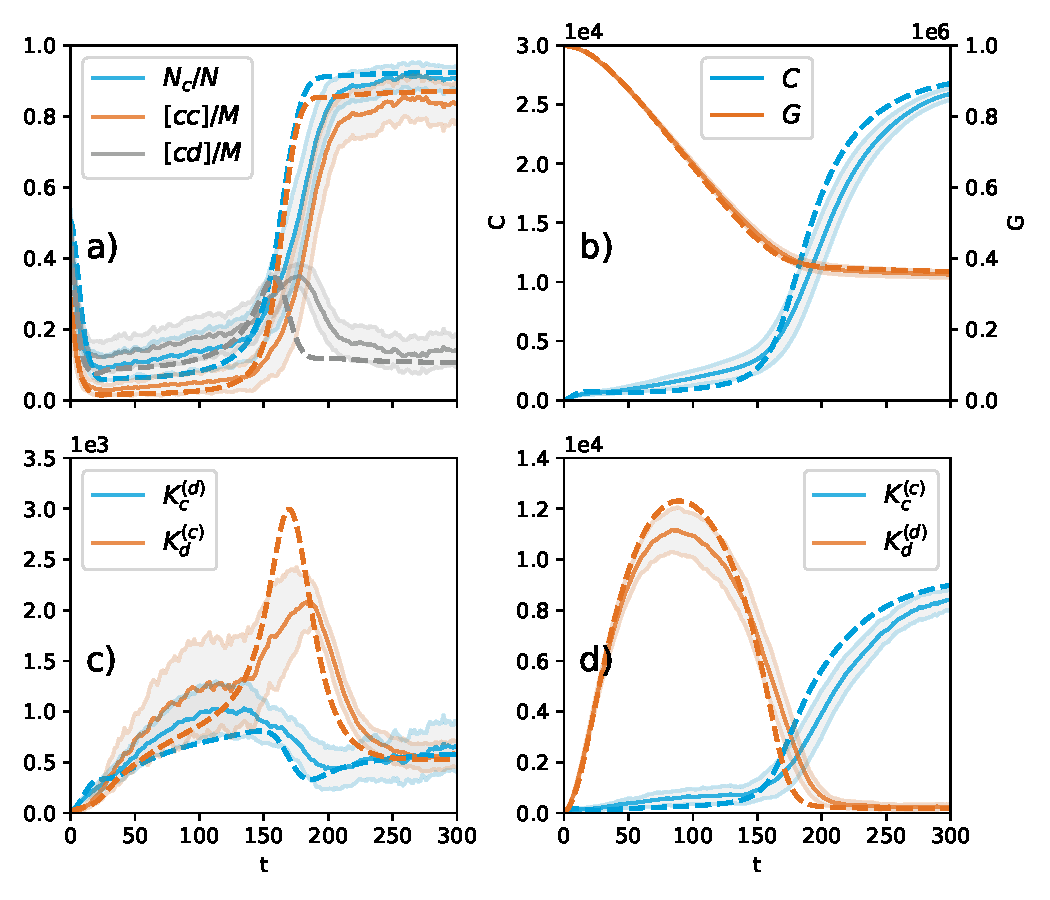
\includegraphics[width=.9\linewidth]{figures/micro_vs_approx_v2.pdf}
\caption{\textbf{Trajectories of dynamic variables from the macro approximation and from measurement in ABM simulations.} The results from ABM simulations (solid lines) are obtained as an ensemble average from 50 runs with standard errors indicated by gray areas. Initial conditions are given by equal shares of the $N=100$ households investing in both sectors and equal endowments in both sectors for all households. The initial acquaintance network amongst the households is an Erd\H{o}s-Renyi random graph with mean degree $k=10$. Other initial conditions are $C_0=0.5$ and $G_0=5 \times 10^5$. All other parameter are given in table \ref{tab:Parameter_list}. The results from the macro approximation (dashed lines of the same colors) are obtained by integration of the ODEs that are obtained from the large system limit with fixed per household quantities. The initial conditions are drawn from the same distribution as previously for the ABM simulations e.g. $N_c$, $[cc]$ and $[cd]$ are calculated from an Erd\H{o}s-Renyi random graph with mean degree $k=10$.}
\label{fig:comparison2}
\end{figure}
%\JK{Maybe better to structure the results as (1), (2), ... and do the same for the full model - then easier to compare}
The results in  fig.~\ref{fig:comparison2} are to some extent complementary to the results in fig.~\ref{fig:example_trajectory} that I discussed in sec.~\ref{sec:numerical_results}. Fig.~\ref{fig:comparison2}d shows capital in both sectors belonging to households that actually invest in these sectors, which is almost equivalent to the variables in fig.~\ref{fig:example_trajectory}d as it makes up almost the entirety of these capital stocks. This can be seen in fig. \ref{fig:comparison2}c: It shows capital of households in the sector that they do not currently invest in, which is approximately an order of magnitude smaller (note the different scale of the y-axis in the figure).

A comparison of the results of the approximation (dashed lines) with those of the numerical simulation of the ABM (solid lines) in fig.~\ref{fig:comparison2} shows that the approximation exhibits the same qualitative features, such as trends, timing and order of magnitude of the displayed variables, as the microscopic model.

Particularly, these results show that for the given parameter values the macroscopic approximation is capable of reproducing very closely the quasi equilibrium states before and after the transition from the dirty to the clean sector, as it lies within the standard error of the ensemble of ABM runs. Also, the approximation is reasonably capable to reproduce the timing of and the transient states during the transition. This is somewhat surprising since in other works, macro-approximations were less well able to get the timing of transition right.

In the following, I discuss the existing differences between the results of the approximated model and the numerical simulation results. 

For instance, I find that the approximation estimates the transition from investment in the dirty sector to investment in the clean sector a bit too early (best visible in panel a). The reason for this might be the slight underestimation of the share of clean investing households, leading to a slight overestimation of the share of dirty capital in the system which is also visible in panel \ref{fig:comparison2}d.

I find a second obvious discrepancy between the micro-model and the approximation in the overestimation of dirty capital of clean investors ($K_d^{(c)}$) (panel c) during the transition phase between $t\approx 150$ and $t \approx 200$. This can be explained by the inequality in capital holdings amongst households. In the approximation, all households investing in dirty or clean capital are assumed to have the same income respectively. Therefore, the probability to change their investment behavior will change for all of them at once during the transition phase leading to a rapid shift of dirty investors changing to invest in clean capital but taking their dirty capital endowments with them (hence the sharp peak in dirty capital of clean investors during the transition phase, see fig.  \ref{fig:comparison2}c dashed grey line). 

Also, in the micro-model, households changing from a dirty to a clean investment strategy take their -- presumably high -- endowments in dirty capital with them. Therefore, the endowments in dirty capital of households investing in the clean sector are relatively wide-spread (see grey area around solid orange line in fig.~\ref{fig:comparison2}c. 
This has effects on the estimated timing of the transition, too. In the micro-model, income of households is heterogeneous. Therefore, for each of them the probability to change their investment behavior changes at different points in time, i.e., poorer households are likely to switch earlier during the transition than richer households. Together this leads to a slower, more spread-out transition dynamic the micro-model resulting in a flatter peak in the dirty capital endowments of clean-investing households.

Another effect at play during the transition is related to the assumptions in equations \ref{eq:neighbordist} and \ref{eq:additional_neighbors}. Namely, that all households that invest in the same type of capital have the same distribution of clean and dirty neighbors.

In the reality of the micro-model, however, these assumptions that are essential to the pair approximation may well be wrong -- especially so during a rapid transition. E.g., a household that has only recently changed its state has a neighborhood that is atypical for its group and adapts only slowly. Consequently, when many changes in the state of the system happen in a short time, a significant proportion of the population is not well described by the assumed approximate distribution.

A number of these effects that lead to discrepancies between the micro-model and the approximation can be mitigated by higher-order moment closure for the distribution of heterogeneous agent-properties or higher-order motif approximation of the network dynamic.

For instance, a higher-order moment closure approximation that tracks the variance and skewness of the distribution of capital endowments can also account for the likelihood of capital endowments of agents that switch their investment decision to be biased. This would presumably mitigate the overestimation of dirty capital of clean investors ($K_d^{(c)}$) during the transition as well as the underestimation of ($K_d^{(c)}$) before the transition and therefore also estimate the timing of the transition even more precisely. 

Similarly, a higher-order motif approximation of the network dynamic can describe the heterogeneity in the local distribution of opinions in the neighborhood of individual agents and correct for the effects of this especially during periods of transient non equilibrium dynamics in the approximated model.\\

In the previous section I derived a set of ordinary differential equations describing the stochastic dynamics of an agent-based model in terms of aggregated variables in the large system limit. I intend this derivation to be a prototypical example for a macroeconomic model with true microfoundations based on heterogeneous agents, given their microscopic interactions are of similar complexity. As such, it might also serve as a starting point for the application and development of similar models for other kinds of social dynamics. For example, an extension to continuous opinions requiring a Fokker-Planck-type description would follow naturally and would grant compatibility to a large body of models for social influence \citep[see ref.][pp. 988 f.]{Mueller-Hansen2017}.

\section{Bifurcation Analysis}
\label{sec:bifurcation-analysis}

The description of the model as a system of ordinary differential equations allows for the analytical analysis of emergent model properties such as multi stability, tipping and phase transitions. 
As a proof of concept application I subsequently show the results of a bifurcation analysis.

\subsection{Methods}
%What is bifurcation analysis?
Bifurcation theory is the analysis of qualitative changes of dynamical systems under parameter variation, for example between a regime with a unique equilibrium (fixed point) and a multi-stable regime.
The parameter value at which a qualitative change, for example in the stability of an equilibrium, occurs is called a critical value or bifurcation point. Bifurcations are classified according to the changes in dynamical properties of the system \cite{Strogatz1994,Kuznetsov1998}.
% Methods for Bifurcation Analysis
Analytical methods have limited scope to identify bifurcation points in non-linear systems. Methods like numerical continuation can handle complex systems of ordinary differential equations like the one derived in Sec.~\ref{sec:Approximation} \citep{Allgower2003}.
Consequently, I use numerical continuation from PyDSTool, a Python package for dynamical systems modeling and analysis \citep{pydstool,10.1371/journal.pcbi.1002628}.\footnote{PyDSTool is building on the AUTO-07p continuation library \citep{Doedel07auto-07p:continuation}.}

% Introduce those kinds of bifurcations that I observe in the analysis:
A common bifurcation type that appears in this model is the fold bifurcation that is also known as saddle-node bifurcation. This type is a local bifurcation in which a stable fixed point collides with an unstable one and both disappear. 
%\JK{Normal form ect. necessary here?} It is described by the normal form $\dot{x} = r + x^2$ with bifurcation parameter $r$. The bifurcation point at $r = 0$ divides a regime with two equilibria for $r < 0$ and a regime without any equilibria for $r > 0$.

Varying two bifurcation parameters at the same time can result in even richer qualitative changes of the dynamics. A prevalent example for such a bifurcation is the cusp geometry \citep[][p.\.397]{Kuznetsov1998}. A change of the second bifurcation parameter in this geometry beyond a certain value results in the so-called cusp catastrophe: the multi-stability of the system disappears for all values of the first bifurcation parameter. As I will show in the following, the macro-approximation of this model indeed exhibits a cusp bifurcation. 

\subsection{Discussion of Results}

\begin{figure}[ht!]
\centering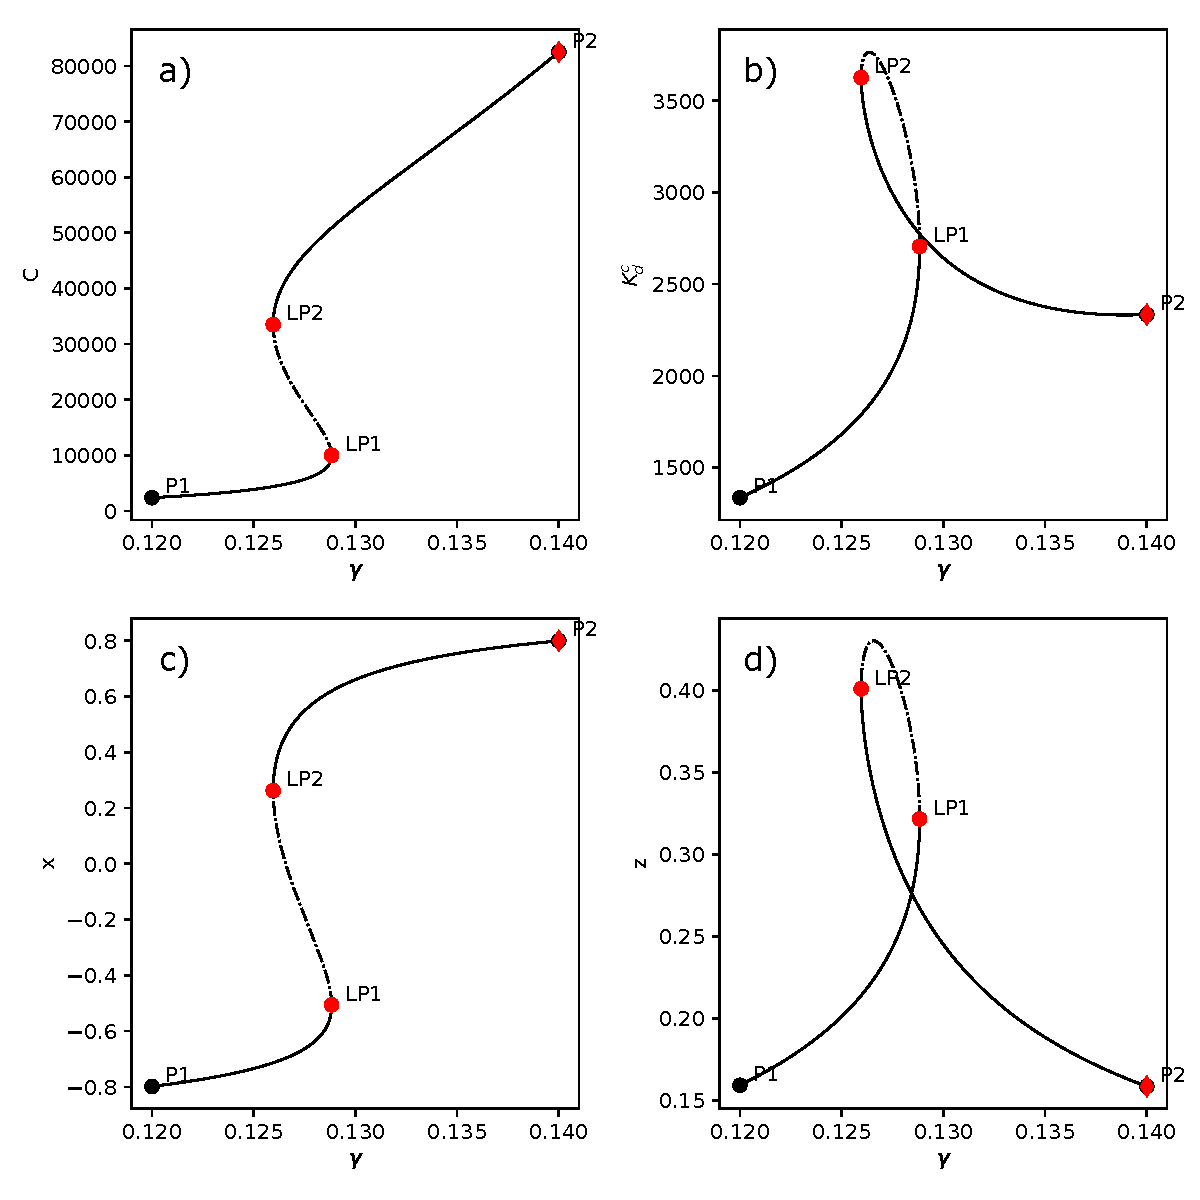
\includegraphics[width=.95\linewidth]{figures/ba_plot.pdf}
\caption{\textbf{Bifurcation diagram:} Continuation of the stationary solution of the macroscopic approximation without resource depletion, e.g. $\dot{G} = 0$ instead of the rate $R$ as given by eq. \eqref{eq:approx_surd}. Bifurcation parameter is $\gamma$, the elasticity of knowledge in the clean sector that also reflects the elasticity of learning by doing of the respective technology. The points labeled P1 and P2 are the beginning and end points of the continuation line, the points labeled LP1 and LP2 are the bifurcation points of two fold bifurcations. The stable unstable manyfold is indicated by a dotted line, the stable manyfold is indicated by solid line. Note that the intersections of the curves in the two right panels do not actually mean that the stationary manifold is not a bijective function of the bifurcation parameter $\gamma$ but rather a result of the projection of the multidimensional manifold onto the two dimensional space.\label{fig:bifurcation_analysis}}
\end{figure}

\begin{figure}[ht!]
\centering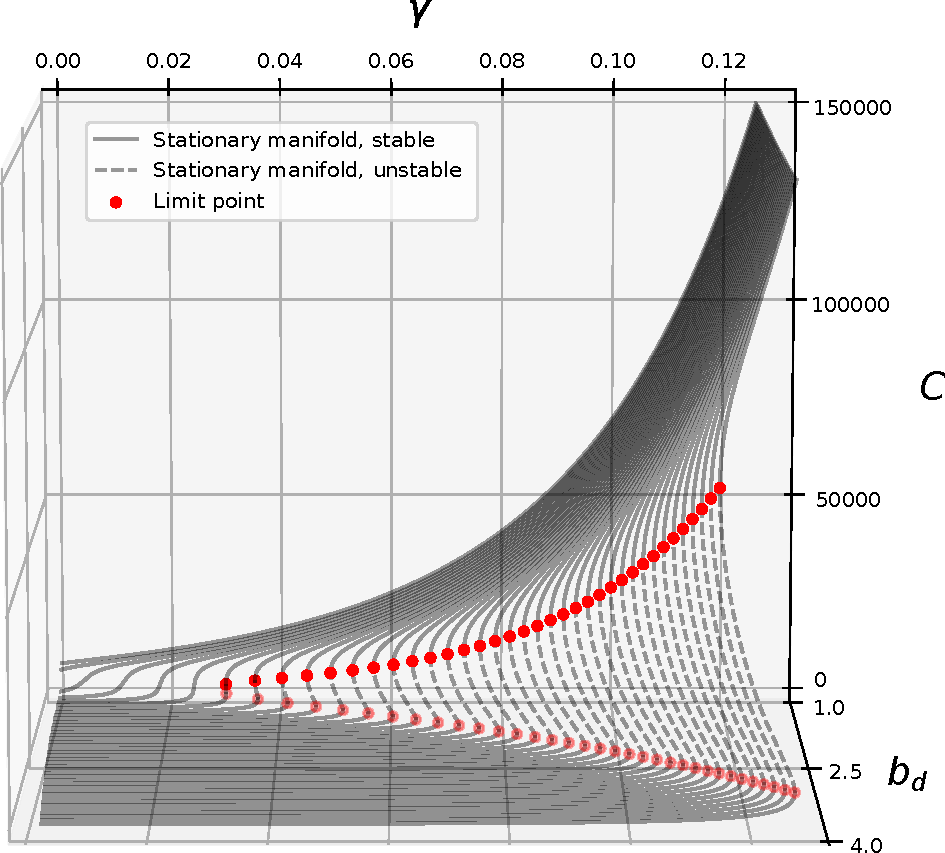
\includegraphics[width=\linewidth]{figures/cusp_better.pdf}
\caption{\textbf{Cusp Bifurcation diagram:}
Stationary manyfold from figure \ref{fig:bifurcation_analysis} panel a for different values of the total factor productivity on the dirty sector $b_d$. Red dots indicate the limit points of the one dimensional fold bifurcation separating the stable and the unstable parts of the stationary manyfold indicated by a solid and a dashed line respectively. For a critical value of $b_d \approx 1.4$ and $\gamma \approx 0.03034$ the two limit points converge and annihilate each other. This codimension two bifurcation with bifurcation parameters $\gamma$ and $b_d$ is called a cusp catastrophe. In this two-sector economic model, this results in a lock in effect in the dirty sector e.g. below this point, there is a smooth transition of production from the dirty to the clean sector and above this point production in the dirty sector is continued even though production in the clean sector would be more efficient. \label{fig:cusp}}
\end{figure}

A considerable advantage of the description of my model in terms of ordinary differential equations \eqref{eq:approx_surd}, \eqref{eq:sum_up_learning} \eqref{eq:lsl_transitions} and \eqref{eq:lsl_capital} over agent based modeling is the fact that it allows for the usage of established tools for bifurcation analysis.
As a proof of concept, I show some results in figure \ref{fig:bifurcation_analysis}.
Here, I analyze the possible steady states of the system with abundant fossil resources e.g. the possible equilibrium states of the model in the regime before the fossil resource becomes scarce and acts as an external driver on the system pushing it towards clean investment.
Therefore, I set the resource depletion to zero e.g. I keep the resource stock in eq. \eqref{eq:approx_surd} constant $G(t) \equiv G_0$ such that the resource usage cost $c_R$ still depends on resource use $R$ but is not increased by deceasing resource stock $G$. Thereby, I eliminate the rising resource extraction cost as the constraint in \cref{eq:approx_equilibrium_wage,eq:approx_dcr} that eventually halts production in the dirty sector. 
I chose the learning rate $\gamma$ as bifurcation parameter as I expect it to yield interesting results.
%That is because as an exponent to a dynamical variable it determines its growth pattern leading to subexponential, exponential or superexponential growth for different values \JK{CITATION NEEDED}. \FMH{I would drop the last sentence because this should be only relevant if I would also consider gamma > 1, but this is certainly not a valid parameter value}.
Generally, in nonlinear dynamical systems, exponential factors are expected to have a strong influence on dynamical properties. Therefore, changing these factors is expected to lead to bifurcation behavior.
Consequently, in figure \ref{fig:bifurcation_analysis} panel a and c I see that for certain learning rates $\gamma$ the macroscopic approximation exhibits a bistable regime limited by two fold bifurcations with bifurcation points indicated by LP1 and LP2.
In this regime both low investment in the clean sector together with hight investment in the dirty sector and low knowledge as well as high investment in the clean sector together with low investment in the dirty sector and high knowledge are stable states of the economic system. This means that in this region economic outcomes are highly path dependent e.g. starting with slightly different knowledge about clean technologies may lead to widely differing adoption levels of the technology in the long run.

Figure \ref{fig:cusp} shows an example of how this bifurcation structure of the dynamical system depends on other parameters. Varying the total factor productivity in the dirty sector $b_d$, the system undergoes a cusp bifurcation. Above a certain value of $b_d$ the system exhibits bi-stability whereas below this value it does not.

%\FMH{Add some words about possible extensions of this analysis?}

Clearly, this choice of bifurcation parameters is only one of many and other choice may very well lead to interesting results. However, I had to limit ourselves to this proof of concept study as an extensive analysis of all possible combinations would be well beyond the scope of this paper.

%\FMH{Do I need this sentence?: Such a configuration would have profound implications on policy design to foster clean technology in order to drive a decarbonization transition in the models production economy.}

Multi-stability of the economy would mean that policies could make use of inherent dynamical properties of the system to reach a desired state or bring the system onto a desired pathway. For example, policy measures such as regulation or taxes can help driving the system into another basin of attraction, i.e. a region of the phase-space in which trajectories approach another equilibrium in the long term. To do so, the system has to cross a separatrix, the boundary between two basins of attraction.
After this boundary is crossed, the policy measure can be discontinued, the system's dynamics guarantee that it reaches the new equilibrium. 
Figure \ref{fig:cusp} shows that such an intervention could be complemented by an additional policy measure, lowering the total factor productivity in the dirty sector, effectively reducing the distance of the stable manyfold from the separatrix and thereby presumably making the first measure less costly.
Another possibility to take advantage of the system's inherent dynamical structure is to use its hysteresis, i.e. to find policy measures that change the first bifurcation parameter $\gamma$ across a bifurcation point or to change the second bifurcation parameter $b_d$ to move the bifurcation point past the current state of the system (or a combination of both) after which the system would fall to the other branch of the stable manyfold. Afterwards, the policy can be discontinued and the system would remain in its new state.
For such considerations, tools from dynamical systems theory and topology can be used to classify the phase-space of the system into regions with respect to the reachability of a desirable state \citep{Heitzig2016,Nitzbon2017}. This allows designing temporary policies that leverage the multi-stability of the socio-economic system.

\section{Discussion and Conclusion}

% Summary: Method
This paper combines a set of methods to overcome shortcomings of current approaches to base macroeconomic models on microfoundations.
While representative agent approaches are unable to capture dynamics that emerge from structured and local interactions of multiple heterogeneous agents, computational agent-based approaches have the disadvantage that they make tractable model analysis difficult and computationally challenging.
I demonstrated that a combination of approximation techniques allows finding a macro description of a multi-agent system in which heterogeneous agents interact locally on a complex adaptive network as well as via aggregated quantities. 
In contrast to previous analytic work, where the network structure was either static \cite{Lux2016}, restricted to star like clusters \cite{DiGuilmi2012} or approximated by a mean field interaction approach and hence neglected \cite{Aoki1998, Aoki2007, Alfarano2008a, DiGuilmi2008, Chiarella2011a}, I explicitly treat the structure of the adaptive complex interaction network with appropriate approximation methods.

I develop a stylized two-sector investment model, in which investment decisions are driven by a social imitation process, to showcase the three approximations:
First, a pair approximation of networked interactions takes into account the heterogeneity in interaction patterns.
Second, a moment closure approximation makes it possible to deal with heterogeneous attributes that characterize the agents.
Third, the large-system limit abstracts from effects due to finite population size.
It is only possible to take this limit if the model has at least one of the following properties: (i) individual interaction depend only on relative rather than absolute quantities such that the size of households can be decreased while taking the number of households to infinity or (ii) the economic production functions exhibits constant returns to scale such that they scale linearly with the number of households $N$.
The resulting set of ordinary differential equations captures the effect of local interactions at the system level while still allowing for analytical tractability.

% Summary: Results
A comparison between a computational version of the ABM and the macro-description reveals that the approximation works well for parameter values distinct from special cases even if only accounting for first moments. Taking more moments into account would increase accuracy but comes at the cost of higher dimensionality and complexity of the macroscopic dynamical system.

% Learnings from model dynamics (topic-wise)
This model shows that social imitation dynamics add inertia to the investment decisions in the system that cannot be captured by a representative agent approach.
The imitation process results in social learning such that agents tend to direct their investments into the more profitable sector over time.
Because of this, the shift of investments from the dirty (fossil) to the clean (renewable) sector is driven only by economic factors, namely increasing exploration and extraction costs for the fossil energy resource.
Thus, I conclude that neutral imitation of better performing peers is not a feasible mechanism to initiate a bottom-up transformation of the economy. Directed imitation, for example driven by changes in social norms, and supporting policies that make dirty production less profitable are needed to initiate a transformation towards a sustainable economy in the absence of fossil resource shortage.

% Why is analytical description desirable
Finding a system of ordinary differential equations to approximate ABMs is useful because it makes the analysis of the dynamical properties of the model much easier. One promising application here is bifurcation theory, as illustrated in Sec.~\ref{sec:bifurcation-analysis}.
Furthermore, it opens the possibility to mathematically proof model properties such as the dependency between different parameters and variables in the model.

% Outlook
% discuss further application 
In the context of climate economics and policy, the proposed techniques are especially important because they allow investigating the interplay of learning agents adapting to new policies and effects of shifts in values and preferences. The resulting changes in individual behavior and their impact on macroeconomic dynamics can be studied in a comprehensive modeling framework. 
Large shifts in investments that are required to reach the goals of the Paris agreement are likely to profit from both, policies that rely on price signals, as well as policies that target individual norm change, interaction and behavior not unlike those researched in e.g. the public health context \cite{Zhang2016, Zhang2015, Centola2011}. The presented techniques can help to better understand how such behavioral interventions would impact the macro-level dynamics of the economic system.

% more specific outlook
%On this regard, there are several promising avenues to develop the model and approximation techniques further: For example, instead of binary opinions, the social interaction model can use continuous variables to represent gradual opinions, drawing on a variety of models of social influence \citep[see ref.][pp. 988 f.]{Mueller-Hansen2017}. An approximation of the agent ensemble would then need a Fokker-Planck-type description rather than a master equation.

% economic modifications
% The model could be extended to explicitly include policy instruments such as a carbon tax and explore its impact on the investment decisions of the heterogeneous agent population. Another promising modification could include consumption decisions into this two-sector model. Consumption decisions are strongly influenced by social norms and interactions \citep{Peattie2010}. Their inclusion could inform the discussion about green consumption as a potential mechanism for a bottom-up transformation towards a more sustainable economy.

% Finally, the techniques proposed in this paper could be used to approximate other systems that interact both locally on a network and in an aggregate way on the system level, for example social-ecological systems or neural networks.
% cite here? \citep{Schlueter2012}

